\section{Video-LDM}
\label{sec:videoldm}

Video-LDM by NVIDIA (2023) \cite{video_ldm} is a text-to-video synthesis model that uses LDM (Latent Diffusion Model, more commonly called Stable Diffusion, section \ref{sec:stable_diffusion}). The main idea of Video-LDM is to first train the model as image generator; and then transform it into a video generator. Its also possible to use pre-trained LDM and then fine-tune it and convert it to a video generator. The model can output in a resolution of up to 1280x2048, which is considered very high resolution in the field of video synthesis.

First, the model is pre-trained with image only datasets; then, temporal layers are added to the LDM that learn to align images in temporally consistent manner; then the model is trained on video datasets and only the temporal layers are learned (the other layers are frozen). They demonstrated that the learned temporal layers can be combined with different image model checkpoints.

\begin{figure}
    \centering
    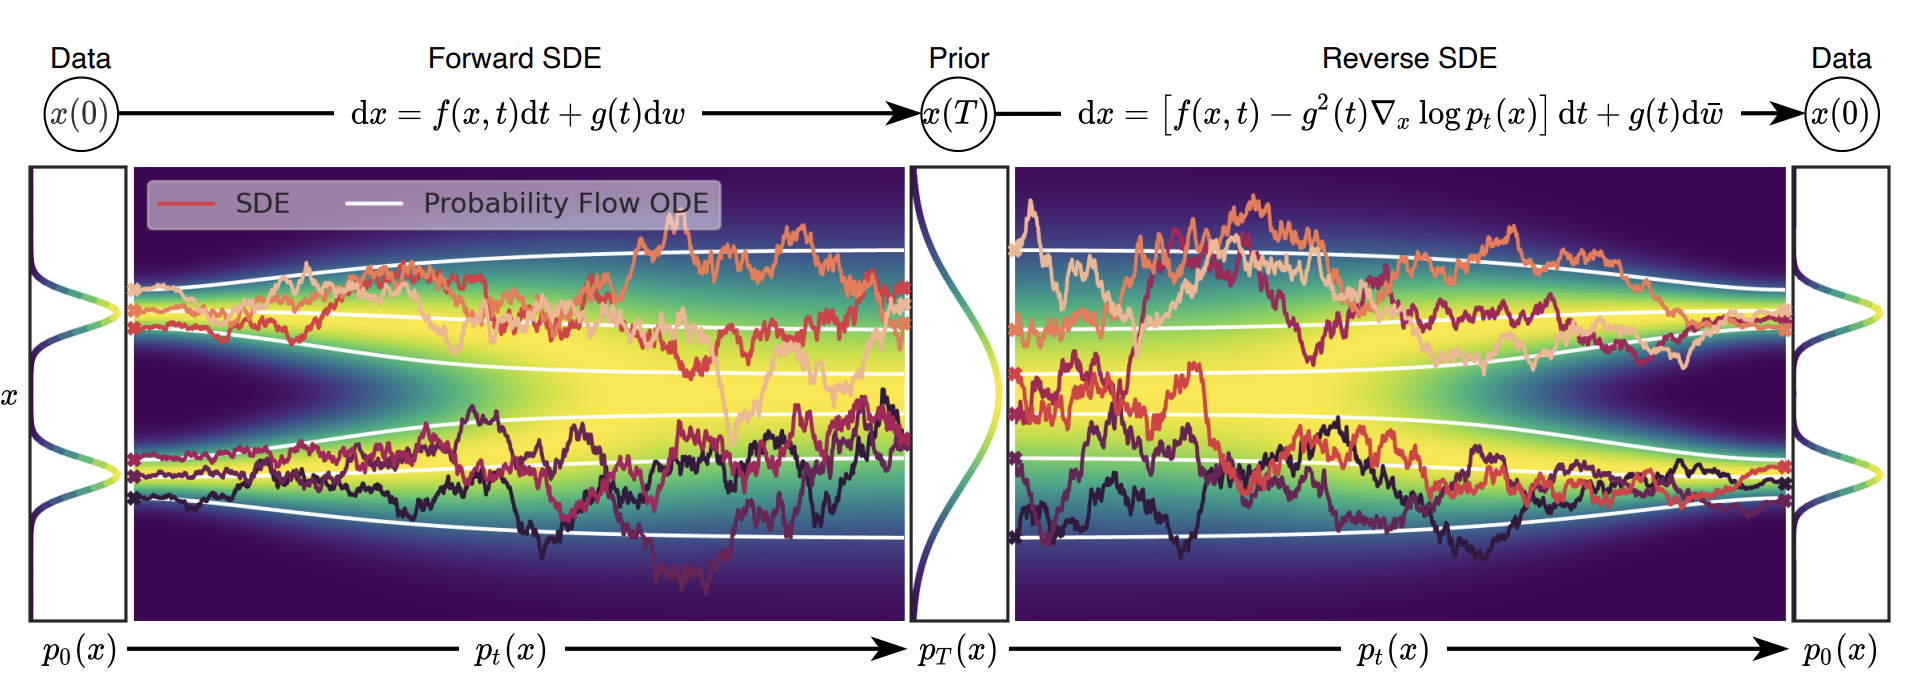
\includegraphics[width=0.8\textwidth]{images/video_ldm/ddpm_sde.png}
    \caption{Generative modeling through stochastic differential equations (SDE) \cite{song2020score}. It shows how data distribution $p(x)$ slowly transforms to prior distribution $p_T(x)$ through forward SDE (we add noise) and then reversed back to generate data with reverse SDE. The colored lines show the SDE paths which represent sample trajectories through the diffusion process. The lines converge at the prior, the noise causes data samples to become progressively less structured, transitioning from a well-defined data distribution to a more chaotic noise-like distribution. The left side shows the probability of the data, the middle shows the probability of the prior (Gaussian distribution), and the right shows we are back to the original data distribution.}
    \label{fig:video_ldm_stochastic}
\end{figure}

\begin{figure}
    \centering
    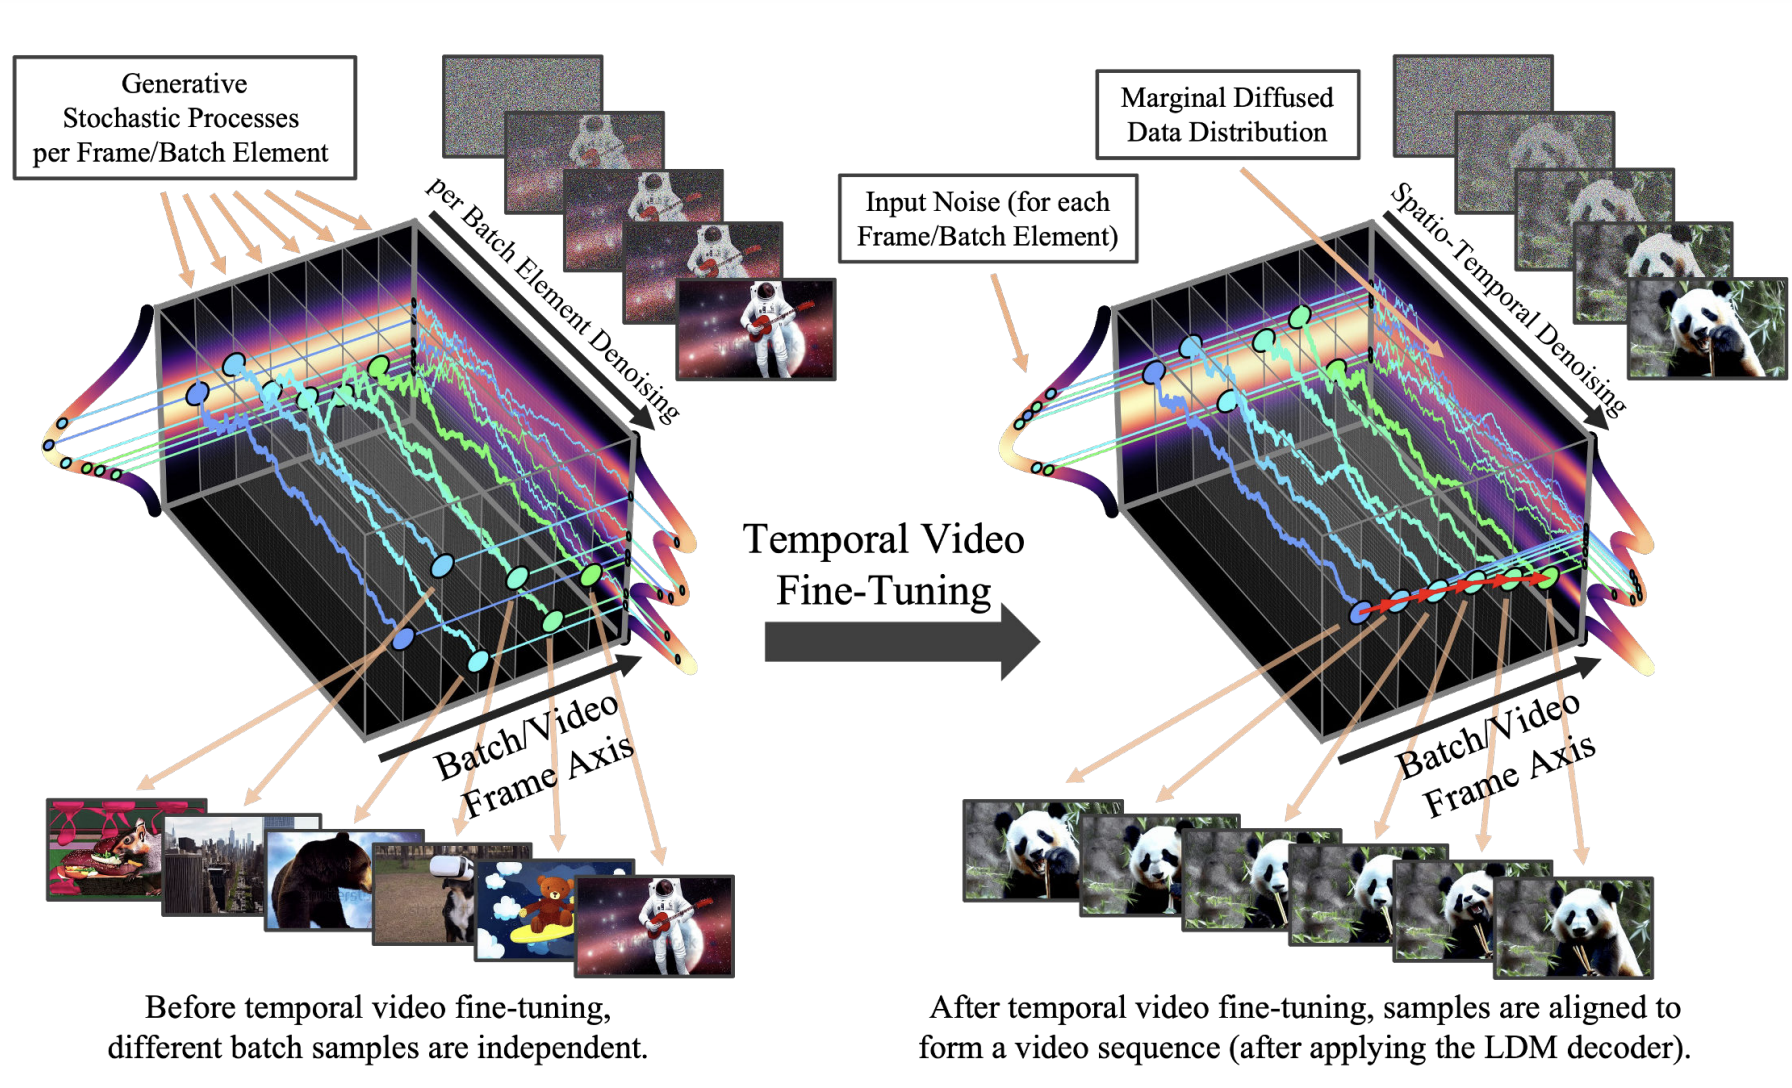
\includegraphics[width=1\textwidth]{images/video_ldm/image_to_video_tuning.png}
    \caption{Transforming image LDM (left) to video LDM (right) \cite{video_ldm}. \textit{Per-batch element denoising}: the stochastic denoising process of diffusion. \textit{Batch/Video Frame Axis}: on the left each image generated is not correlated to other images in the batch; on the right each generated image is correlated to the previous image, the model learns to align them and generate temporally consistent video. \textit{Batch/Video Frame Axis}: the red arrows and line shows how one image transitions to the next image, creating the video.}
    \label{fig:video_ldm_image_to_video_tuning}
\end{figure}

\subsection*{Mathematical notations}

The LDMs autoencoder compresses the high-dimensional input data $x \in \mathbb{R}^{T \times 3 \times \hat{H} \times \hat{W}}$ where $x \sim p_{\text{data}}$ is a sequence of $T$ RGB frames with height $\hat{H}$ and width $\hat{W}$ to lower-dimensional latent space $z = \mathcal{E} (x) \in \mathbb{R}^{T \times C \times H \times W}$ (where $C$ is the number of latent channels, and $H, W$ are the spatial latent dimensions) in order to improve computational needs. The model then learns to reconstruct $x$ via decoder $\mathcal{D}$: $\hat{x} = \mathcal{D} (\mathcal{E} (x)) \sim x$.

Let us denote the layers of the LDM (without temporal layers) as spatial layers $l^i_{\theta}$ where $\theta$ are the model's parameters, and $i$ is the layer index. We then denote the addition of temporal layers as $l^i_{\phi}$ to learn to align individual frames in a temporally consistent manner. We denote $f_{\theta, \phi}$ as the full model (with spatial and temporal layers).

\subsection{Architecture}

...

\begin{figure}
    \centering
    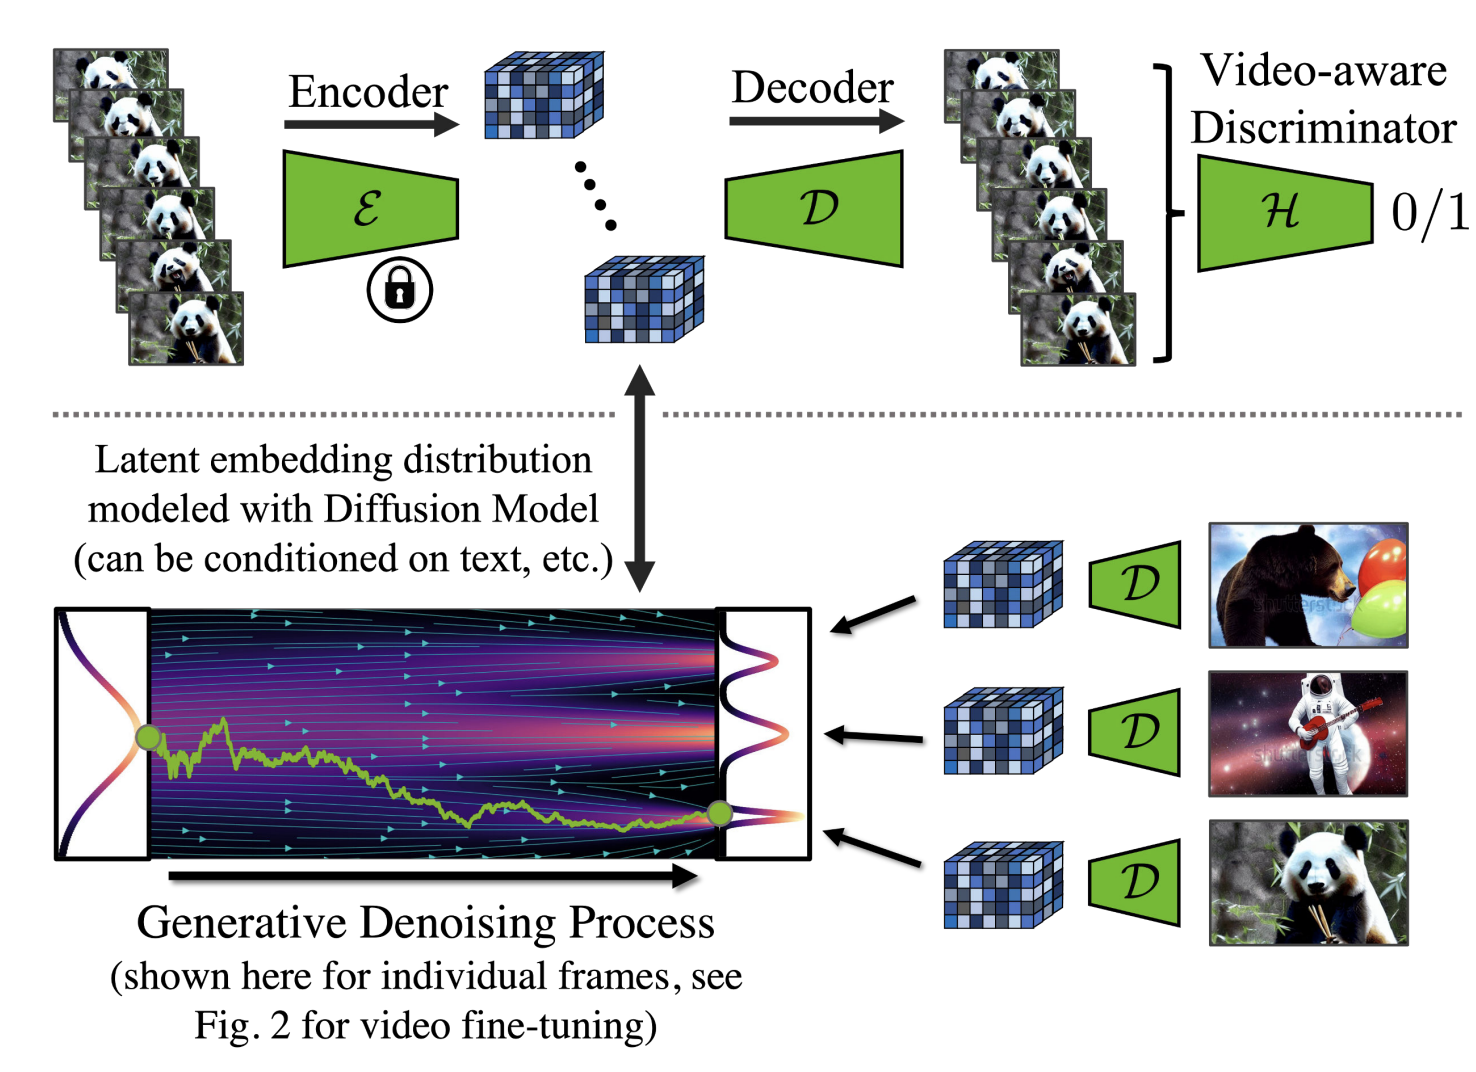
\includegraphics[width=0.7\textwidth]{images/video_ldm/enc_dec_denoise_process.png}
    \caption{Top: frozen encoder compresses video frames into 3D latents and the decoder learns to reconstruct image from the latent (like in autoencoders). The patch-based discriminator $\mathcal{H}$ is used to increase photorealism, the adversarial objective is added to the autoencoder reconstruction score like in PatchGAN (\cite{isola2017image} which tries to classify if $N \times N$ patch is real or fake). \textit{Bottom}: generative denoising process, each embedding corresponds to different image generation in the decoder $\mathcal{D}$.}
\end{figure}



\begin{figure}
    \centering
    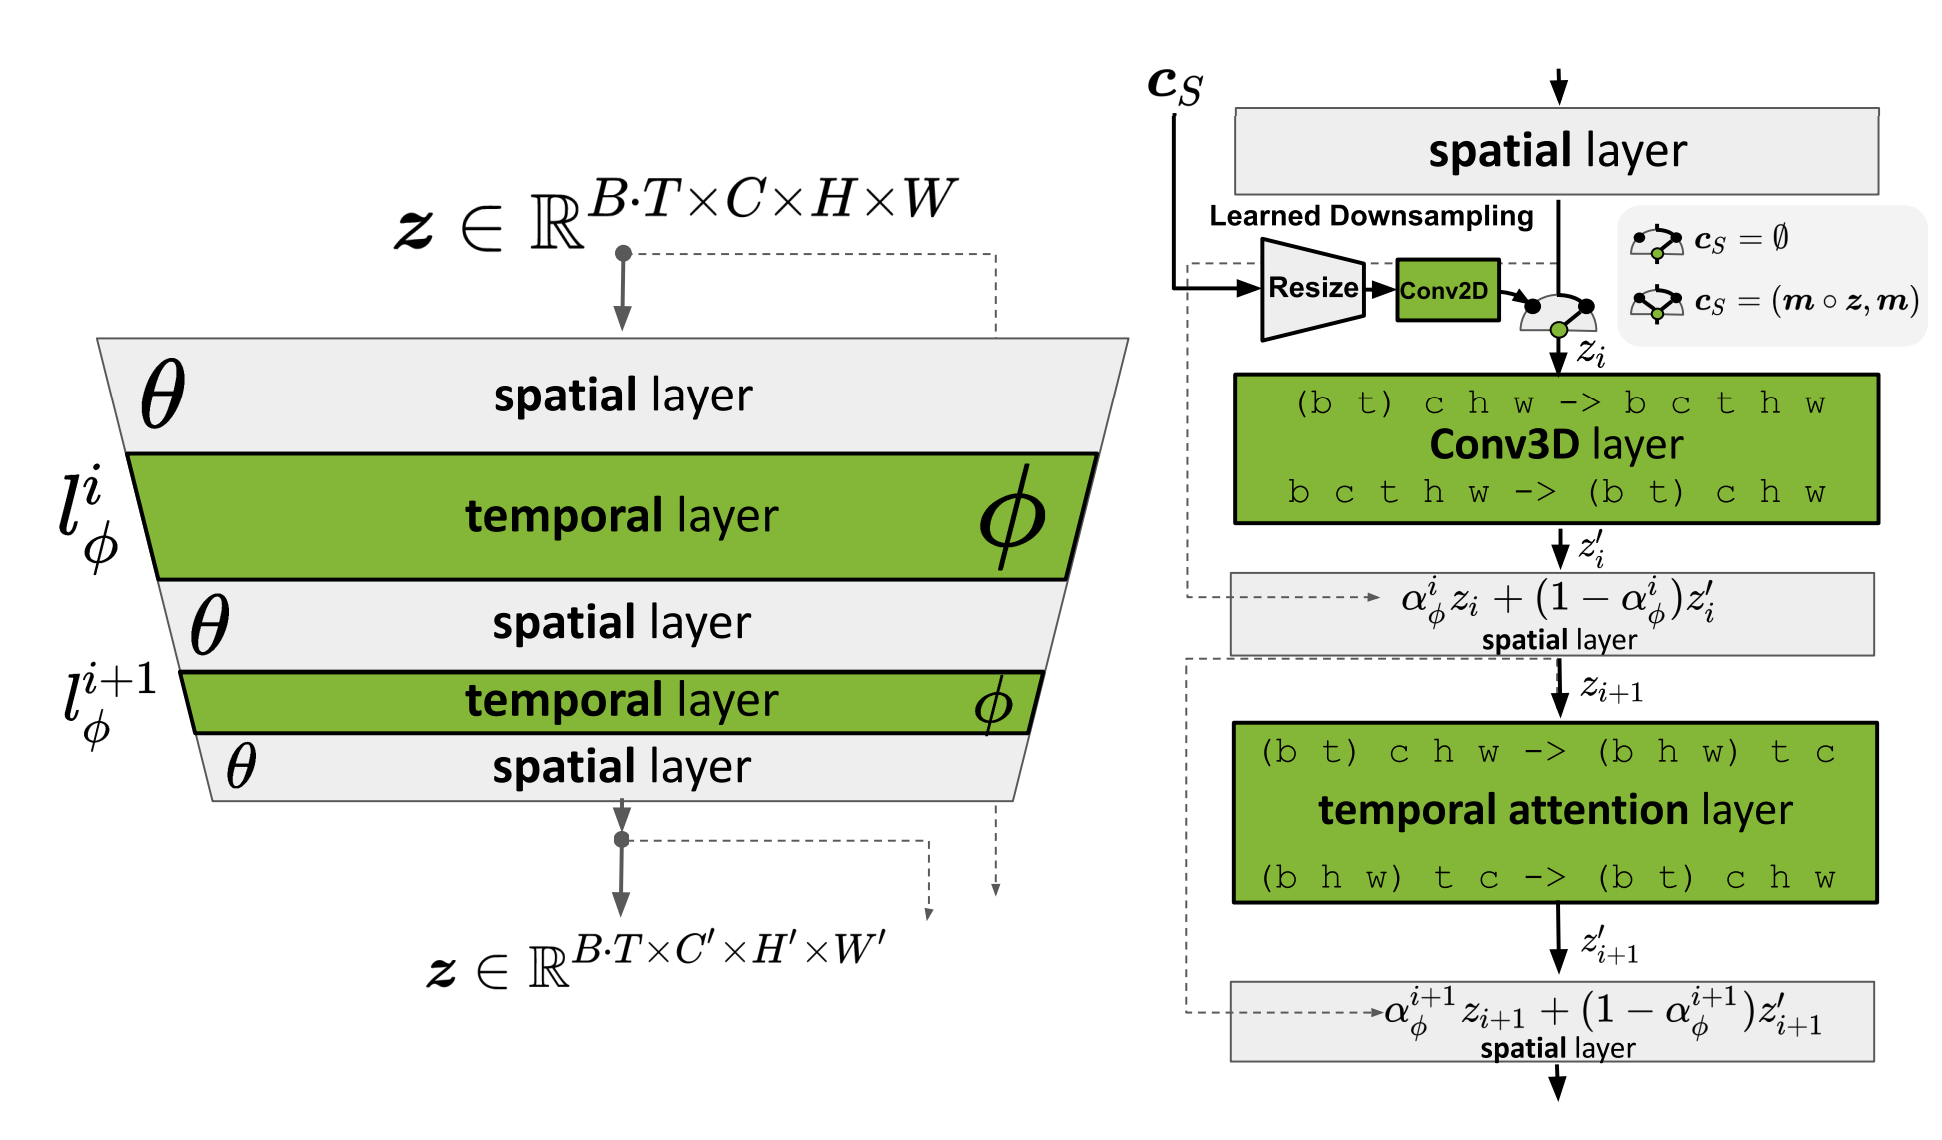
\includegraphics[width=0.7\textwidth]{images/video_ldm/temporal_layers.png}
    \caption{\textit{Left:} The researchers turn pre-trained LDM into video generator by adding temporal layers $l_\phi$ that learn to align images in a temporally consistent manner. The spatial layers $l_\theta$ are frozen and only the temporal layers are learned. \textit{Right:} }
\end{figure}


